% RLJ main.tex Version 2026.1
\documentclass[10pt]{article} % For LaTeX2e

\usepackage{rlj}           % Should be uncommented for submission
%\usepackage[accepted]{rlj} % Should be uncommented for the camera-ready
%\usepackage[preprint]{rlj} % Should be uncommented for preprint versions

%%%%%%%%%%%%%%%%%%%%%%%%%%%%%%%%%%%%%%%%%%%%%%%%%%%%%%%%%%%%%%%%
% Recommended (but not required) packages
%%%%%%%%%%%%%%%%%%%%%%%%%%%%%%%%%%%%%%%%%%%%%%%%%%%%%%%%%%%%%%%%
\usepackage{amssymb}
\usepackage{mathtools}
\usepackage{amsthm}
\usepackage{mathrsfs}
\usepackage{graphicx}
\usepackage{booktabs}
\usepackage{url}

%%%%%%%%%%%%%%%%%%%%%%%%%%%%%%%%%%%%%%%%%%%%%%%%%%%%%%%%%%%%%%%%
% Theorem environments and macros
%%%%%%%%%%%%%%%%%%%%%%%%%%%%%%%%%%%%%%%%%%%%%%%%%%%%%%%%%%%%%%%%
\theoremstyle{definition}
\newtheorem{definition}{Definition}
\theoremstyle{plain}
\newtheorem{theorem}{Theorem}
\newtheorem{lemma}{Lemma}
\newtheorem{proposition}{Proposition}

\newcommand{\Ex}{\mathbb{E}}
\newcommand{\Hist}{\mathcal{H}}
\newcommand{\Acts}{\mathcal{A}}
\newcommand{\ModE}{\mathcal{M}_E}
\newcommand{\PiK}{\Pi_{K_L}}
\newcommand{\Vlow}{V^{\mathrm{lo}}_t}
\newcommand{\Vhi}{V^{\mathrm{hi}}_t}
\newcommand{\Rex}{\mathcal{R}^{\mathrm{ex}}}
\newcommand{\Rmax}{R_{\max}}
\newcommand{\Dstruct}{\Delta^{\mathrm{str}}}

%%%%%%%%%%%%%%%%%%%%%%%%%%%%%%%%%%%%%%%%%%%%%%%%%%%%%%%%%%%%%%%%
% Meta-data (cover page) -- fill in the TODO fields
%%%%%%%%%%%%%%%%%%%%%%%%%%%%%%%%%%%%%%%%%%%%%%%%%%%%%%%%%%%%%%%%
\title{TODO}

\setrunningtitle{TODO}

\author{Anonymous Authors\textsuperscript{1}}

\emails{anon@example.com}

\affiliations{
$^{1}$\textbf{Anonymous Institution}
}

\contribution{TODO}{None}

\keywords{TODO}

\summary{TODO}

\begin{document}

\makeCover
\maketitle

\begin{abstract}
TODO
\end{abstract}

\section{Introduction}
\label{sec:intro}

\section{Position}

Short summary of position

\section{Definition}
\label{sec:defs}


We work over a single, never-resetting stream of experience and assume no Markov, episodic, or stationarity structure. Rewards lie in $[0,\Rmax]$, and we measure value over an $H$-step look-ahead. The agent is capacity-bounded: it represents policies and beliefs within a fixed budget of bits. We seek a definition of a learning measure the agent can compute from its own state, the condition under which it is trustworthy, and the limit beyond which it cannot be.

\begin{definition}[Stream, policy, value]
\label{def:basic}
A \emph{history} is $h_t = (o_0,r_0,a_1,\dots,a_t,o_t,r_t)$, with observations $o_s$, rewards $r_s \in [0,\Rmax]$, actions $a_s$; the underlying law is $\mu$. A \emph{policy} $\pi$ maps histories to action distributions, with value $f^{\pi}_t = \Ex_{\mu,\pi}\!\big[\sum_{s=t+1}^{t+H} r_s \mid h_t\big]$.
\end{definition}

\begin{definition}[What the learner could have done]
\label{def:capcomp}
The learner represents policies within $K_L$ bits; write $\PiK$ for this representable set. The \emph{within-capacity optimum} is $f^{K_L}_t = \sup_{\pi \in \PiK} f^{\pi}_t$, and the \emph{structural gap} to the global optimum is $\Dstruct_t = f^{*}_t - f^{K_L}_t \ge 0$. We compare the agent to $f^{K_L}_t$, the best it could itself express, and keep $\Dstruct_t$ visible as the irreducible price of being small.
\end{definition}

\begin{definition}[Learner and examiner]
\label{def:agent}
An agent is a pair $(\mathcal{L},\mathcal{E})$. The \emph{learner} $\mathcal{L}$ emits the policy $\pi_t \in \PiK$ it acts with, and learns only about that policy. The \emph{examiner} $\mathcal{E}$ is a \emph{predictive model}: from the history it outputs an \emph{aspiration} $\Vhi$ and a \emph{guarantee} $\Vlow$, with $\Vhi \ge \Vlow$. Setting $\Vhi$ requires forecasting the value of policies the learner did not run, so the examiner must learn about a whole family of behaviours, not the one acted. In the spirit of general value functions \citep{sutton2011horde,modayil2014nexting}, temporally abstract predictions \citep{suttonprecupsingh1999}, and off-policy prediction \citep{precup2001offpolicy}, $\Vhi$ and $\Vlow$ are value predictions the agent learns from its own stream, and the examiner's \emph{inductive bias}, the model class $\ModE$ of environments it considers possible, the concentration rule, or the prior of its predictors, is what lets it generalize to behaviours it has not tried. A Bayesian posterior over a model class is one instance, not the only one \citep{osband2013psrl}.
\end{definition}

\begin{definition}[Examiner regret]
\label{def:exreg}
$\rho_t = \Vhi - \Vlow \ge 0$, with $\Rex_T = \sum_{t=1}^T \rho_t$. It depends only on the history and the examiner; it never refers to $\mu$ or to any optimum.
\end{definition}

\section{A Worked Case: The Examiner in a Bandit}
\label{sec:bandit}

The simplest world in which the definitions become concrete has no state at all. A multi-armed bandit is the stream of Section~\ref{sec:defs} with $|\mathcal{S}|=1$ and $H=1$. We use it for two reasons: it is the standard sanity check for any value-based definition, and it makes ``a behaviour the learner never tried'' as transparent as possible, namely an arm it never pulled.

\paragraph{Setting.} There are $N$ arms; pulling arm $i$ returns a reward $r\in\{0,1\}$ with unknown mean $\mu_i$, so $\Rmax=1$. Every arm pays $\tfrac12$ except a single \emph{special} arm with $\mu_{i^\star}=\tfrac12+\epsilon$, and the agent acts on one never-resetting stream. Write $\hat\mu_i$ for the empirical mean of arm $i$, $n_i$ for its pull count, and $c_i=\sqrt{2\ln t/n_i}$ for the confidence half-width, with $c_i$ at its maximum for an arm never pulled.

\paragraph{The definitions become arithmetic.} With $H=1$ the value of the policy ``pull arm $i$'' (Definition~\ref{def:basic}) is the arm mean, $f^{\pi}_t=\mu_i$. If every arm is representable, the within-capacity optimum (Definition~\ref{def:capcomp}) is $f^{K_L}_t=\mu^\star=\tfrac12+\epsilon$ and the structural gap vanishes, $\Dstruct_t=0$. The learner $\mathcal{L}$ selects the played arm $a_t$; the examiner $\mathcal{E}$ (Definition~\ref{def:agent}) reads its two numbers off the same counters,
\[
\Vhi=\max_i\big(\hat\mu_i+c_i\big),
\qquad
\Vlow=\hat\mu_{a_t}-c_{a_t},
\]
an optimistic ceiling over \emph{all} arms and a pessimistic floor on the \emph{played} arm, with inductive bias $\ModE$ equal to the concentration rule that lets $c_i$ shrink with data. The examiner regret (Definition~\ref{def:exreg}) is then the confidence width,
\[
\rho_t=\Vhi-\Vlow=\max_i\big(\hat\mu_i+c_i\big)-\big(\hat\mu_{a_t}-c_{a_t}\big),
\]
which uses only counts and empirical means, never $\mu$ or $\mu^\star$. These are not new objects: $\sum_t(f^{K_L}_t-f^{\pi_t}_t)=\sum_t(\mu^\star-\mu_{a_t})$ is the classical pseudo-regret and $\sum_t\rho_t=O(\sqrt{NT\log T})$ is the standard UCB confidence-width sum \citep{auer2002ucb,lai1985asymptotically}.

\paragraph{Where honesty lives.} Call the examiner \emph{sound} if its floor is a true floor, $\Vlow\le f^{\pi_t}_t$, and its ceiling a true ceiling, $\Vhi\ge f^{K_L}_t-\delta_t$; by Hoeffding both hold with high probability, with slack $\delta_t$ the failure margin that vanishes as counts grow. The mechanism is one line: an arm never pulled keeps $c_i$ at its maximum, so its optimistic index stays high and the ceiling $\Vhi$ cannot fall. The examiner is structurally forbidden from reporting ``no room to improve'' about an arm it has not inspected; a dishonest examiner is exactly one that discards this and assumes the unseen arm is ordinary.

\paragraph{Three behaviours (Figure~\ref{fig:bandit}).} First, a self-report alone certifies nothing: a trivial examiner reporting $\rho_t\equiv0$ pairs equally with a good (UCB) learner and a bad (fixed-arm) learner, identical reports but opposite true regret (panel~A). Second, when the world is coverable ($N=5$), a sound $\sum_t\rho_t$ stays above the true within-capacity regret throughout, a valid if loose certificate of what remains removable (panel~B). Third, when the world outruns the horizon ($N>T$) and the special arm is placed out of reach, a sound examiner honestly keeps $\rho_t$ large, signalling uncovered ground, while a biased examiner that assumes a shared mean collapses $\rho_t$ toward zero and reports a false ``done'' even as true regret climbs at rate $\epsilon$ (panel~C). This last case is the price the position pays in a big world: an honest, vanishing self-report is not free.

\begin{figure}[t]
\centering
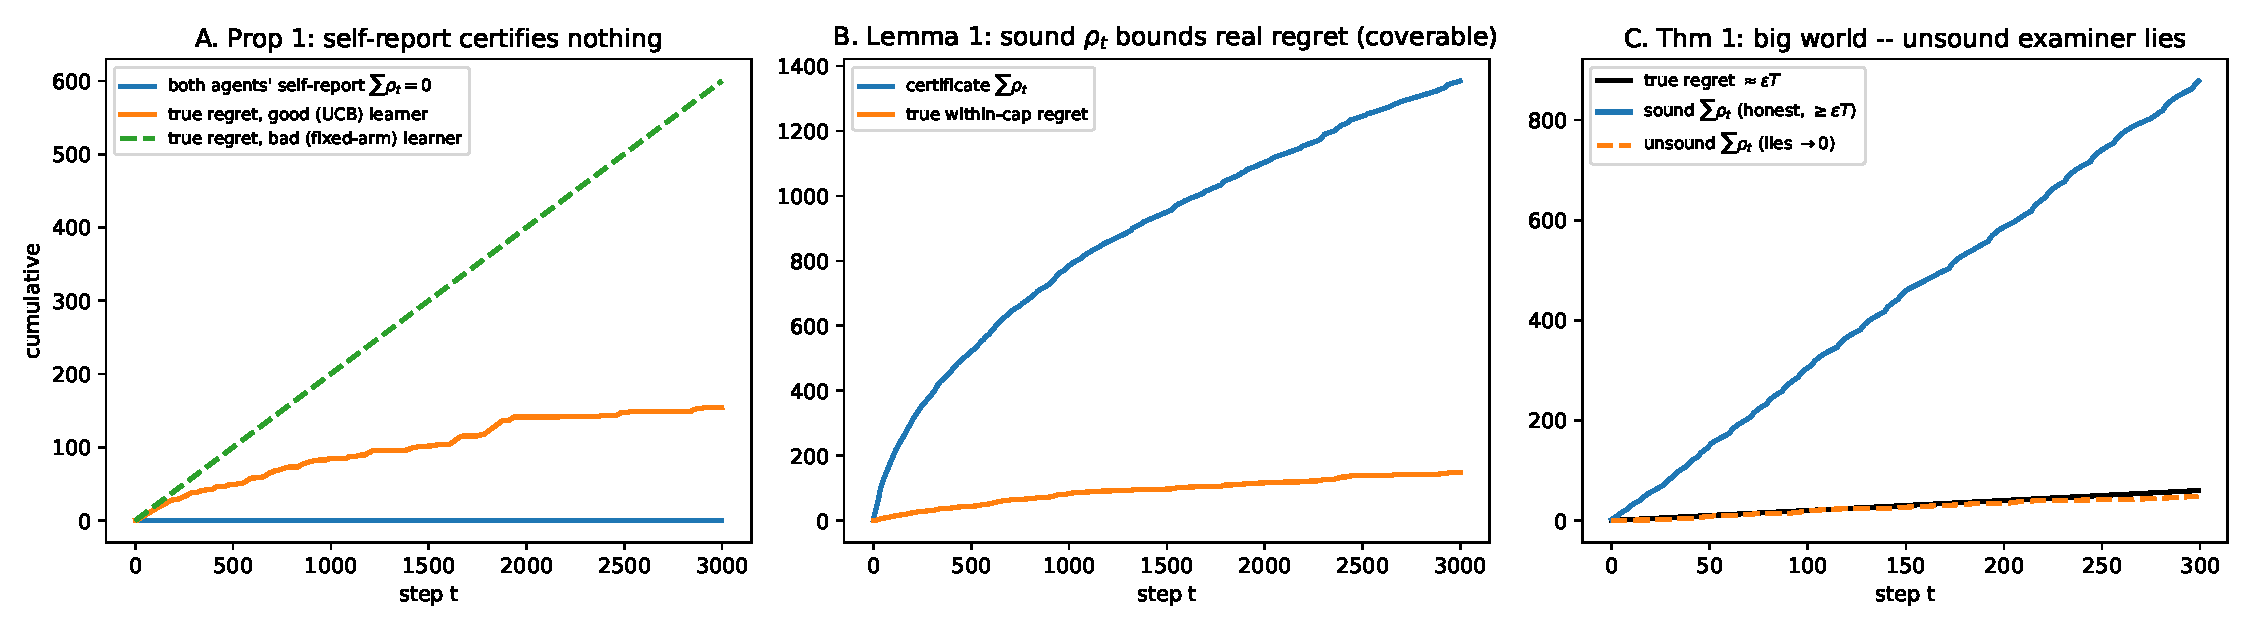
\includegraphics[width=\textwidth]{examiner_bandit_demo.pdf}
\caption{The examiner in a bandit. \textbf{(A)} Two agents with the identical self-report $\sum_t\rho_t=0$ differ arbitrarily in true regret. \textbf{(B)} In a coverable world the sound certificate $\sum_t\rho_t$ upper-bounds the true within-capacity regret. \textbf{(C)} When the world outruns the horizon, a sound examiner keeps $\rho_t$ large (honest), while a biased examiner drives $\rho_t$ below the true regret (unearned confidence).}
\label{fig:bandit}
\end{figure}

\paragraph{How to use it.} The bandit shows the three intended uses without any external optimum. As a \emph{monitor}, $\rho_t$ is an online read of self-assessed room to improve; as a \emph{comparison metric}, two algorithms on one stream are ranked by which $\rho_t$ shrinks faster toward its capacity-constrained optimum; and as an \emph{audit}, a low $\rho_t$ is trustworthy exactly on the covered region, with the big-world case above marking when no audit is possible and apparent convergence should instead trigger exploration or external testing.

\bibliography{main}
\bibliographystyle{rlj}

\end{document}
